
The baseline solution for the Distance Network  as illustrated in Figure~\ref{fig:baseline_DN} yields 
\begin{equation}
H_0 = \Hvaluebase \pm \Herrorbase \, \Hunit~.
\end{equation} 
As described in Section~\ref{sec:define_baseline}, this solution includes SNe~Ia, SBF, and megamaser measurements as Tracers. The distances to hosts of SNe~Ia and SBF calibrators are obtained from the solution of the full \DN, incorporating measurements based on TRGB and Cepheids from the sources described in Section~\ref{sec:data_summary}, with the Milky Way, LMC, and NGC$\,$4258 as anchors for Cepheid distances.\footnote{Note that the current version only uses TRGB measurements for the calibration of the SBF method, in accordance with the most recent publication \cite{2025ApJ...987...87J}; in future iterations we intend to allow for arbitrary primary distance indicators for the calibration.} SNe~Ia measurements are from the Pantheon+ sample, and peculiar velocity corrections in the Hubble flow are based on the 2M++ model \citep{2015MNRAS.450..317C}.  This solution has an overall $ \chi^2 $ of {\redchisqbase} per degree of freedom, indicating broad agreement between the estimated uncertainties---all based on original sources---and the statistical properties of the solution.  Note that the value of $ \chi^2 $ does not include degrees of freedom associated with SNe~Ia and SBF tracers in the Hubble flow. In our methodology, we solve separately for the Hubble flow intercept for SNe~Ia and SBF tracers in the Hubble Flow---as well for others that are not included in the baseline solution, such as SNe~II and TF tracers---and only the intercept is included in the final \DN{} solution. It can be shown that, apart from a separation of the $\chi^2$ values, this approach is equivalent to directly including the Hubble tracer equations into the {\DN}; see also Appendix~\ref{app:sec:intercept}.

\begin{figure}
    \centering
    \includegraphics[width=\textwidth]{Figures/LocalDistanceNetwork_Baseline.png}
    \caption{The Baseline Distance Network, illustrated analogously to Fig.\,\ref{fig:DN_full} \label{fig:baseline_DN}}
\end{figure}

\begin{figure}
    \centering
    \includegraphics[width=0.9\linewidth]{Figures/ISSI-H0-Workshop-DistanceNetwork-baseline-batlowKS.pdf}
    \caption{Residuals for each category of host distance measurements from the Baseline solution.  Each panel represents a group of measurements of host distances that share the same method, anchor, and authors, and shows the deviation of those measured host distances from the full distance network value.  Error bars represent the individual uncertainty of each measurement, while the shaded regions for each group shows the common (fully correlated) uncertainty due to the reference system.}  
    \label{fig:baseline_residuals}
\end{figure}

Figure~\ref{fig:baseline_residuals} shows the residuals of host distances, estimated from the network solution, grouped by methodology. 
Each grouping, identified by a different color, refers to a specific combination of primary distance indicator, anchor, and source, as indicated in the labels below the group. The error bars shown correspond to the uncertainty of the specific distance measurement for that host, not including terms that are covariant with the other elements of the group. For example, each Cepheid measurement is shown with the uncertainty of the Period-Luminosity intercept for that galaxy, which reflects the expected scatter of residuals \textit{within that group}.  The color-shaded band for each group shows instead the uncertainty associated with common error terms for that group, i.e., the anchor uncertainty and the uncertainty in the indicator measurement (TRGB magnitude or Cepheid Period-Luminosity intercept) for that anchor, combined in quadrature; this term is indicative of the likely scatter of the \textit{average} of the group---shown by the corresponding horizontal line at the center of the band---with respect to zero.\footnote{This is a slightly simplified description of the uncertainties, as it accounts for most, but not all, covariances in the data. However, it is a useful guide to the properties of residuals, as long as the formal $ \chi^2 $ is consistent with the statistics of the system.}  As can be seen, the distribution of residuals is consistent with expectations, with no significant deviation from the published uncertainties for any subset of data.  

A closer look at the residuals for Cepheids shows clearly that all anchors are consistent with one another \textit{and} with TRGB; the systematic offsets (horizontal bars) for Cepheids anchored to the LMC, the Milky Way, and NGC$\,$4258 differ by 0.02 mag or less from the distance network solution.  Subsets of TRGB measurements have slightly larger typical offsets, about 0.03 mag, justified in part by the smaller number of systems included in each study; but overall they are in very good agreement, within the expected statistical uncertainties. 

\begin{figure}
    \centering
    \includegraphics[width=0.9\linewidth]{Figures/ISSI-H0-Workshop-HubbleFlow-baseline-batlow25-Log.pdf}
    \caption{Residuals in distance modulus as a function of redshift for objects in the Hubble flow in the Baseline solution.  Error bars reflect the individual source scatter, without the common calibration uncertainty.  The shaded region in each plot indicates the effect of a velocity uncertainty of $ 250 \, \mathrm{km \, s^{-1}} $.  The bars at the right show the mean and dispersion for each group of sources and the calibration uncertainty, which is a common error mode for all points in each panel.} 
    \label{fig:baseline_hf}

\end{figure}

Figure~\ref{fig:baseline_hf} shows the distribution of residuals for objects in the Hubble flow as a function of redshift for three classes of objects.  The ordinate is the offset in $ \log_{10}{(H_0)} $ inferred for that specific object; the error bar reflects a combination of the measurement uncertainty (photometric error, error in standardization, and/or uncertainty in the solution, as applicable), the effect of the dispersion in peculiar velocities, the uncertainty in the peculiar velocity reconstruction, and the intrinsic dispersion in the relevant distance indicator, as determined in the original sources from the dispersion in the calibrators. They do not include the calibration uncertainty, which is determined as part of the distance network calibration solution for each group when applicable.  The shaded bars at the right show the measured mean and dispersion for each of the three sets of data. Again, both the dispersion in individual measurements and the mean for each subset are consistent with expectations, which represent the direct measurement uncertainties for each value---not including calibration uncertainties.  Figure~\ref{fig:baseline_corner} shows the posterior distribution for the global fit parameters for this solution: the absolute magnitude calibration for SNe Ia, the offset in the SBF calibration, the estimated distances to Virgo and Fornax, and the value of {\Hcst}.  These are based on finite-length chains extracted from the probability distribution of the solution, and the values of the parameters may be slightly different from the analytically calculated results.

\begin{figure}
    \centering
    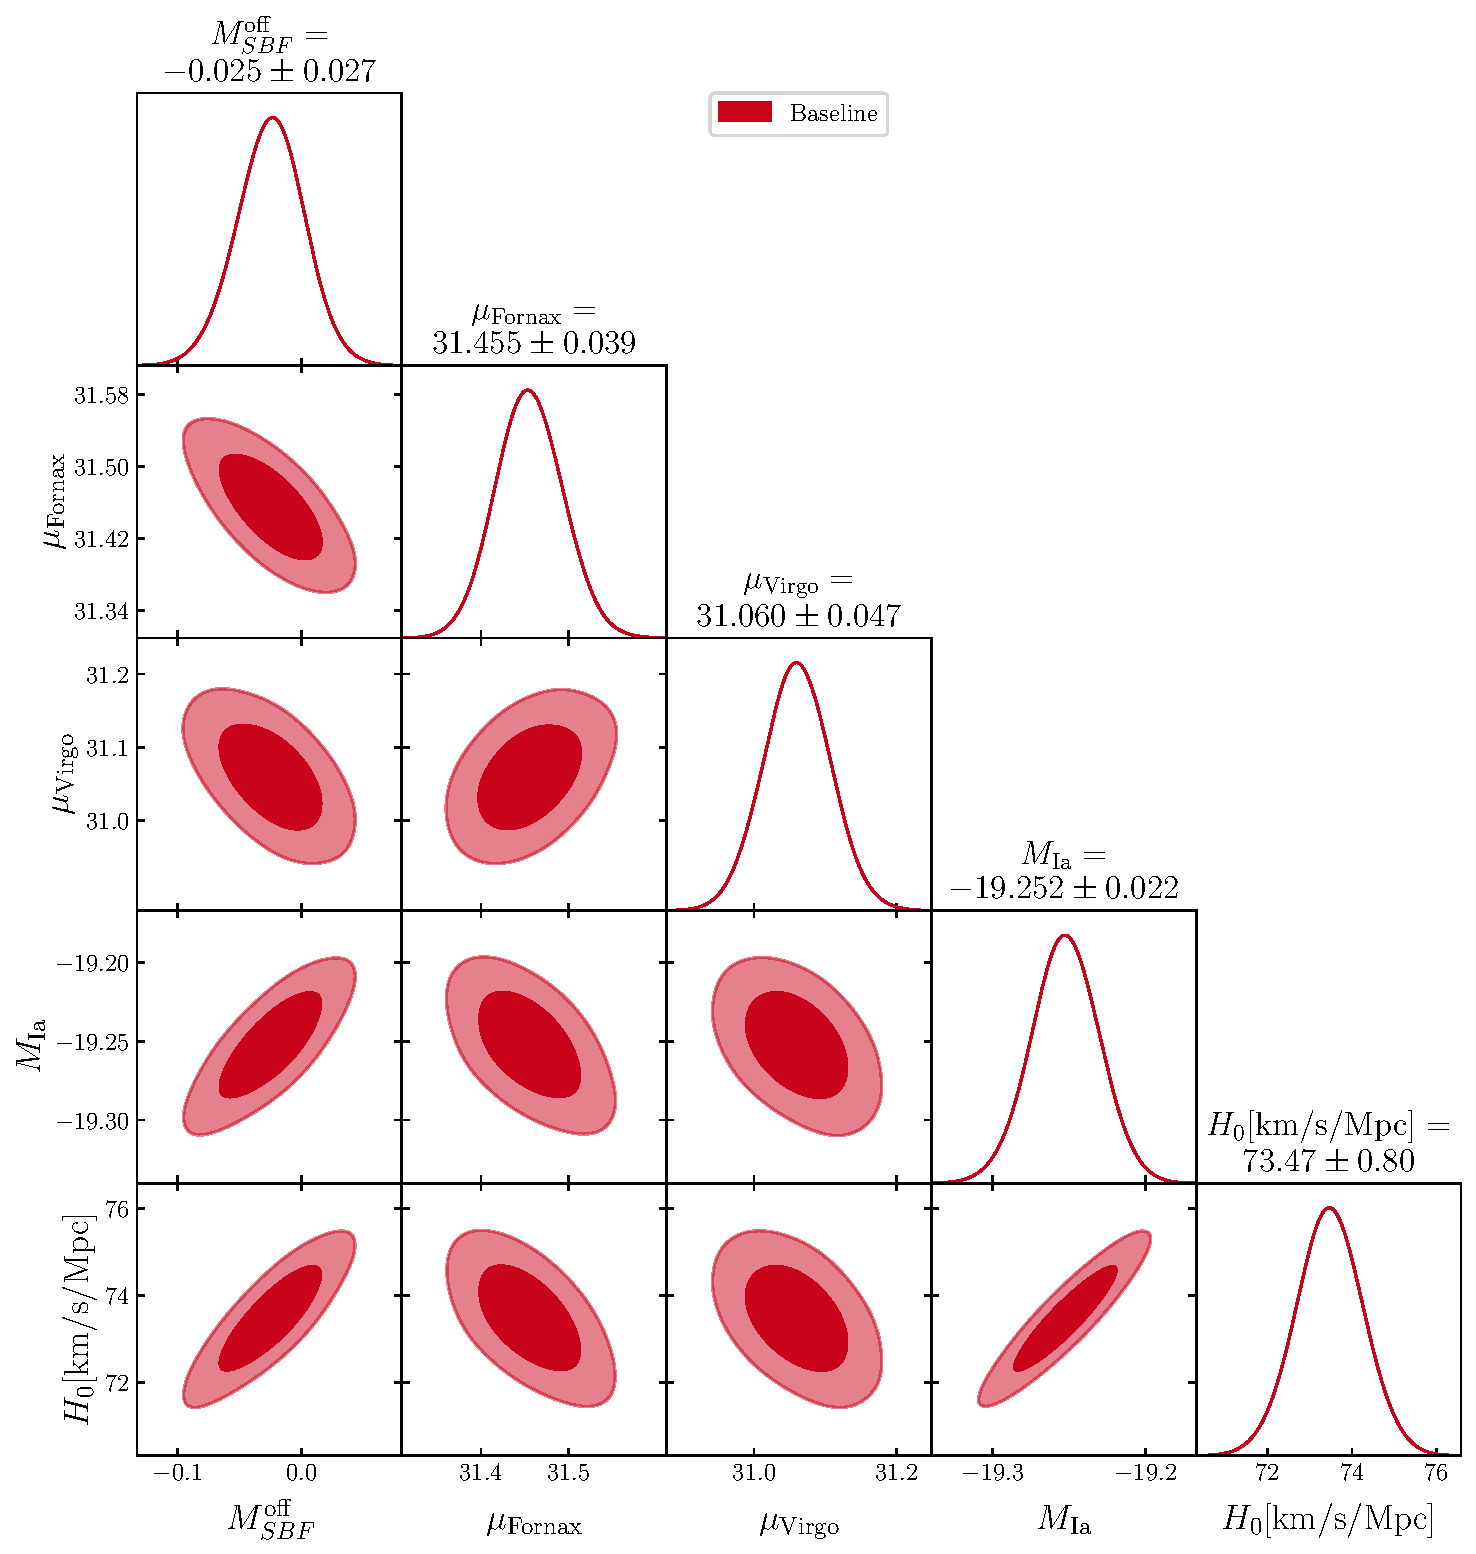
\includegraphics[width=0.9\linewidth]{Figures/chains_base_title_forpub.pdf}
    \caption{Corner plot for the baseline solution, illustrating the correlations between {\Hcst}, the calibration of SNe~Ia and SBF, and the distance to Fornax and Virgo, which contribute to the SBF calibration. The parameters use the naming convention of Appendix~\ref{sec:optimization_parameters}. Deviations from the analytically calculated result are due to the numerical precision of a finite-length chain.}
    \label{fig:baseline_corner}
\end{figure}

The solution for the baseline {\DN} yields the most accurate direct {\Hcst} measurement to date, with a relative uncertainty of \Hrelerrorbase, including systematic uncertainties. It agrees to much better than the $1\sigma$ uncertainty with previous determinations of {\Hcst} by the SH0ES team \citep{2022ApJ...934L...7R}.

The relative uncertainty of this result improves by  $\gtrsim 13\%$ over updates by the SH0ES team based on cluster Cepheids \citep{2022ApJ...938...36R} and sibling SNe~Ia \citep{2023JCAP...11..046M}, and by $\sim 7\%$ compared to the most recent SH0ES update provided by \citet{2024ApJ...973...30B}, which furthermore incorporated the SMC as an additional anchor. As shown by \citet{2022ApJ...934L...7R}, integrating TRGB distances into the fit strengthens the result, but does not cause it to deviate strongly. In the baseline case, this finding extends to the inclusion of distant megamasers and the SBF measurements. More generally, we find excellent agreement with most previous literature results based on direct measurements, as we show in Fig.~\ref{fig:whiskerCMB}---including most of the studies corresponding to the individual distance ladders that can be constructed within the {\DN}. We explicitly investigate the similarities and differences with respect to previous literature results that are part of the {\DN} in Appendix~\ref{sec:comparisons}, where we also showcase what is necessary to obtain the results with lower central values in \Hcst\,. We also find great agreement with the recent TDCOSMO results from \citet{2025arXiv250603023T}, which give $\Hcst = 71.6^{+3.9}_{-3.3}\Hunit$ and are compatible at $\sim0.5 \sigma$.

The consensus \Hcst{} measurement differs from the indirect, $\Lambda$CDM-dependent, measurement based on the CMB anisotropies of $\Hvaluecmb \pm \Herrorcmb \,\Hunit$ \citep[][Eq.~(54)]{2025arXiv250620707C} at a statistical significance of $\Hsigmabase \sigma$. 

\begin{figure}
    \centering
    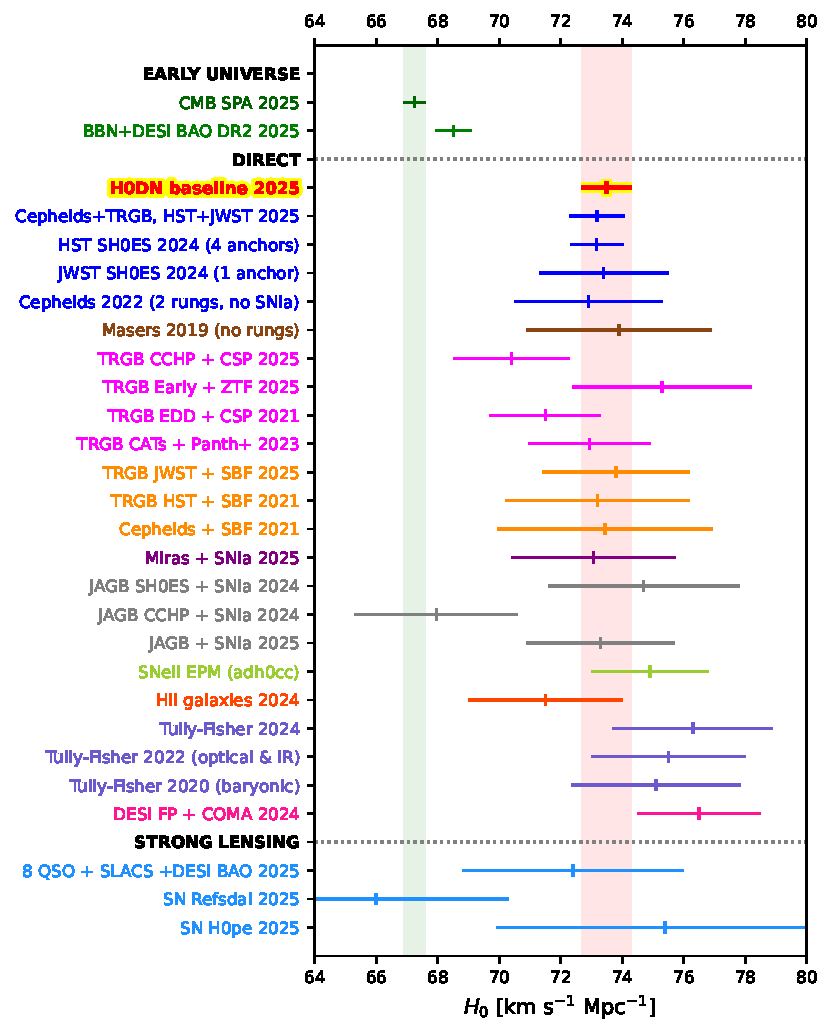
\includegraphics[width=0.8\linewidth]{Figures/H0_whisker_CMB.pdf}
    \caption{Comparison of the baseline result with  previous literature results, based on early universe indirect inferences using the flat $\Lambda$CDM model, based on direct measurements in the late universe, and based on strong lensing results (which involve additional modeling).
    }
    \label{fig:whiskerCMB}
\end{figure}
